Alla luce delle funzionalità che gli emulatori di rete oggi esistenti offrono, desideriamo, con l'obiettivo di approfondire le nostre conoscenze in ambito di reti e di sviluppo software, proporre una soluzione alternativa che offra feature extra ed un miglioramento generale della qualità di utilizzo.
\newline\newline
L'architettura della piattaforma proposta è stata ideata come segue:
\begin{center}
    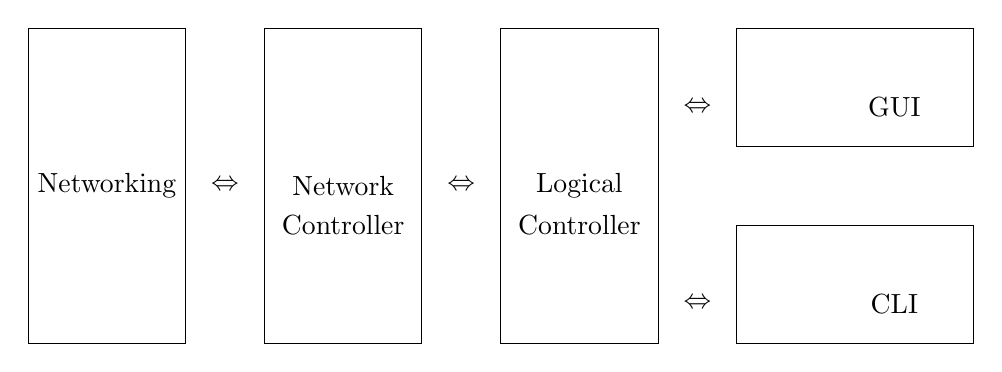
\begin{tikzpicture}
        \draw (12,0) rectangle (15, 1.5);
        \draw (12,2.5) rectangle (15,4);
        \draw (11,0) rectangle (9,4);
        \draw (8,0) rectangle (6,4);
        \draw (3,0) rectangle (5,4);
        \node[] at (4,2) {Networking};
        \node[] at (7,2) {Network};
        \node[] at (7,1.5) {Controller};
        \node[] at (10,2) {Logical};
        \node[] at (10,1.5) {Controller};
        \node[] at (14,0.5) {CLI};
        \node[] at (14,3) {GUI};
        \node[] at (5.5,2) {$\Leftrightarrow$};
        \node[] at (8.5,2) {$\Leftrightarrow$};
        \node[] at (11.5,0.5) {$\Leftrightarrow$};
        \node[] at (11.5,3) {$\Leftrightarrow$};
    \end{tikzpicture}
\end{center}

Per tanto, le componenti da realizzare sono:
\begin{itemize}
    \item \textbf{Networking}: Utilizzo di container e apparati virtualizzati. Si tratta del modo in cui vengono realizzati, come in IMUNES, i componenti veri e propri. Essi sono poi connessi tra di loro mediante gli appositi comandi e possono simulare una rete. Sarà gestito dal relativo controller attraverso utilizzo di librerie apposite sviluppate ad hoc.
    \item \textbf{Network Controller}: Automatizzazione, a fronte di una topologia creata, della creazione della configurazione di rete
    \item \textbf{Logical Controller}: Logica di controllo, a più alto livello, che possa gestire:
          \begin{itemize}
              \item Strutture per gestire la topologia creata
              \item Salvataggio della topologia
              \item Gestione e salvataggio delle configurazioni
              \item Invio delle informazioni necessarie al network controller per realizzare la topologia creata
          \end{itemize}
    \item \textbf{GUI}: si tratta dell'interfaccia su cui l'utente può disegnare la topologia logica della rete, posizionando quindi nodi e link tra nodi, trascinandoli, modificandoli e interagendoci in genere
    \item \textbf{CLI}: da qui si possono lanciare i comandi di configurazione dei vari componenti. Essa aprirà un editor di testo sui file di configurazione, permettendo quindi di modificarli, salvarli e caricare le modifiche anche nella visualizzazione GUI. Permetterà di accedere a CLI dedicate ai singoli nodi per inserire configurazioni
\end{itemize}
Gli obiettivi che desideriamo perseguire attraverso questo progetto sono:
\begin{itemize}
    \item \textbf{Ridurre le dipendenze} al minimo necessario, in modo da rendere il programma il più portabile possibile
    \item Fornire la \textbf{capacità di salvare} non solo la topologia fisica ma anche tutte le configurazioni, senza bisogno di script ulteriori
    \item \textbf{Uscire in modo pulito}, evitando che Docker rimanga in uno stato intermedio (ossia con i vecchi container ancora presenti) in caso di chiusura della applicazione senza arresto della simulazione
\end{itemize}



\newpage
